\documentclass[12pt, a4paper]{article}

\usepackage{amsmath}
\usepackage{array}
\usepackage{amsmath}
\usepackage[portuguese]{babel}
\usepackage{chngpage}
\usepackage{float}
\usepackage[a4paper, margin=2cm]{geometry}
\usepackage{graphicx}
\usepackage{hyperref}
\usepackage{listings}
\usepackage{setspace}
\usepackage{xcolor}

\lstdefinestyle{codestyle}{
    commentstyle=\color{teal},
    keywordstyle=\color{blue},
    numberstyle=\ttfamily\color{gray},
    stringstyle=\color{red},
    basicstyle=\ttfamily\footnotesize,
    breakatwhitespace=false,
    breaklines=false,
    keepspaces=true,
    numbers=none,
    showspaces=false,
    showstringspaces=false,
    showtabs=false,
    tabsize=4
}
\lstset{style=codestyle}

\title{\Huge \textbf{Computação Gráfica \\ \Large Trabalho Prático -- Fase II}}
\date{30 de março 2025}
\author{Grupo 3}

\begin{document}

\begin{center}
    
\includegraphics[width=0.25\textwidth]{res/cover/EE-C.eps}
\end{center}

\chardef\_=`_
\onehalfspacing
\setlength{\parskip}{\baselineskip}
\setlength{\parindent}{0pt}
\def\arraystretch{1.5}

{\let\newpage\relax\maketitle}
\maketitle
\thispagestyle{empty}

\vspace*{\fill}

\begin{adjustwidth}{-2cm}{-2cm} % These values only need to be large enough to center the table
    \begin{center}
        \begin{tabular}{>{\centering}p{0.25\textwidth}
                        >{\centering}p{0.25\textwidth}
                        >{\centering}p{0.25\textwidth}
                        >{\centering\arraybackslash}p{0.25\textwidth}}
            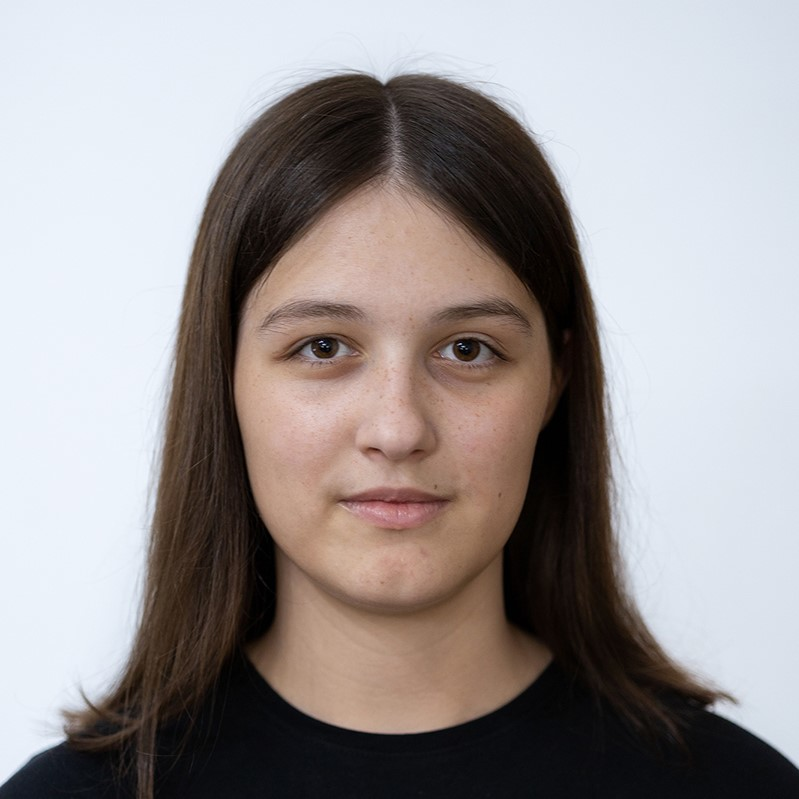
\includegraphics[width=3.5cm]{res/cover/A104437.png} &
            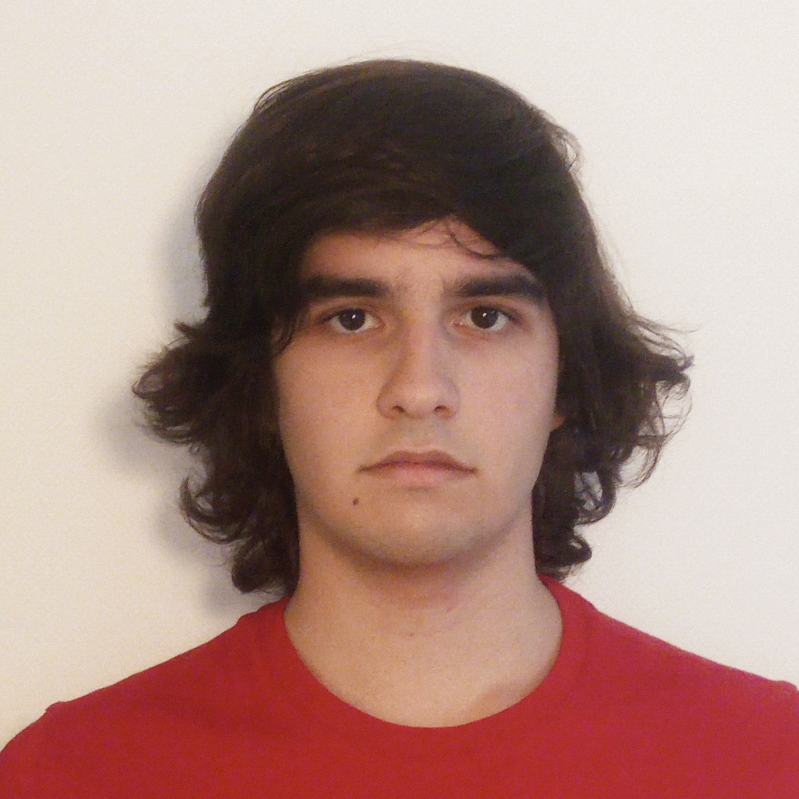
\includegraphics[width=3.5cm]{res/cover/A104348.png} &
            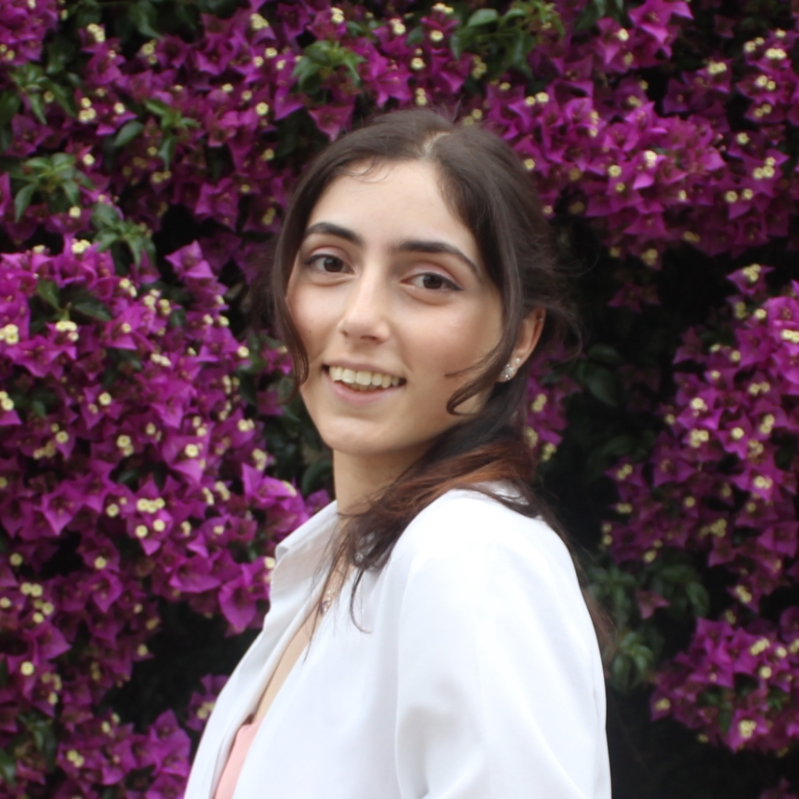
\includegraphics[width=3.5cm]{res/cover/A90817.png} &
            
\includegraphics[width=3.5cm]{res/cover/A104179.png} \\

            Ana Oliveira & Humberto Gomes & Mariana Cristino & Sara Lopes \\
            A104437      & A104348        & A90817           & A104179
        \end{tabular}
    \end{center}
\end{adjustwidth}

\pagebreak

\begin{abstract}
    \textbf{\color{red} TODO - resumo}
\end{abstract}

\section{Transformações}

\textbf{\color{red} TODO - transformações}

\section{Modelo estático do sistema solar}

\textbf{\color{red} TODO - sistema solar}

\section{Extras}

\section{\emph{Frustum culling}}

Cada \emph{draw call} tem um custo elevado para o desempenho da aplicação. Logo, procurando reduzir
o número de \emph{draw calls}, foi implementado \emph{frustum culling}, para apenas ser requisitada
à GPU a renderização dos objetos no \emph{view frustum} da câmara.

Seria muito computacionalmente intensivo verificar se a geometria de um modelo se encontra dentro ou
fora do \emph{view frustum}, pelo que se encapsulam todos os modelos em esferas que, devido à sua
geometria simples, permitem uma verificação rápida da sua visibilidade no \emph{view frustum}. No
entanto, visto que estas esferas podem ser um pouco maiores do que os modelos em si, é possível que
alguns objetos fora do ecrã sejam desenhados, visto que parte das suas esferas ainda intersetam os
planos do \emph{view frustum}. Para mitigar este problema, formas geométricas encapsuladoras mais
complexas poderiam ser utilizadas, visto que estas poder-se-iam melhor adaptar à geometria dos
modelos. No entanto, o uso destas formas complexas conduziria a testes de visibilidade mais caros,
possivelmente anulando os benefícios de desenhar um menor número de objetos.

Quando um modelo é carregado, é necessário calcular a esfera que o encapsula. Em primeiro lugar, o
seu centro é calculado como o centro de massa de todos os pontos, como mostra a expressão abaixo,
onde $M$ é o modelo, uma sequência de pontos tridimensionais:

$$
C = \frac{1}{|M|} \sum_{p \in M} p
$$

Depois, o raio da esfera pode ser determinado como a distância entre o centro da esfera e o ponto
mais longínquo do mesmo, como mostra a expressão abaixo, onde $d$ define a função entre dois pontos:

$$
r = \max \left \lbrace d(C, p) \mid p \in M \right \rbrace
$$

É também necessário saber como uma esfera encapsuladora é afetada quando o objeto que encapsula
sofre uma transformação no mundo. Considere-se uma matriz de transformação aplicada ao objeto (em
coordenadas do mundo), originada através da aplicação de translações, rotações, e escalas. A matriz
terá dimensões 4x4 e o seguinte aspeto:

$$
\bgroup
    T =
    \begin{bmatrix}
        \vec \imath & \vec \jmath & \vec k & \vec t \\
        0 & 0 & 0 & 1
    \end{bmatrix}
\egroup
$$

Para calcular o centro da esfera após a transformação da entidade, basta multiplicar a matriz de
transformação pela posição do centro da esfera:

$$
C' = T C
$$

Depois, para calcular o novo raio da esfera, não é necessário ter em conta as transformações de
rotação, visto que as esferas são simétricas em todos os eixos possíveis. No entanto, é necessário
ter em conta a escala aplicada ao modelo. Por exemplo, na matriz $T$, a escala da entidade pelo
eixo $x$ é $\lVert \vec \imath \rVert$, e o mesmo se tem para o $y$ e $\lVert \vec \jmath \rVert$ e
para $z$ e $\lVert \vec k \rVert$. Logo, o raio da esfera transformada é:

$$
r' = \max(\lVert \vec \imath \rVert, \lVert \vec \jmath \rVert, \lVert \vec k \rVert) \cdot r
$$

É possível tirar proveito da estrutura hierárquica da cena para otimizar o processo de
\emph{frustum culling}. Por exemplo, caso um grupo contenha várias entidades ou subgrupos, pode
construir-se uma esfera que encapsula a totalidade do grupo. Caso essa esfera não esteja no
\emph{view frustum}, pode-se evitar fazer os testes de visibilidade para as esferas dos objetos
individuais que compõe o grupo. Caso contrário, é na mesma necessário realizar esses testes.

O processo para determinar as características de uma esfera que encapsula todos os objetos de um
grupo é semelhante ao da construção de esferas com base no conjunto de pontos de um modelo. Em
primeiro lugar, para determinar o centro da esfera, calcula-se o centro de massa do conjunto de
pontos formado pelos centros de todas as esferas, $C$. De seguida, para cada subesfera, calcula-se
a sua distância máxima a $C$, a distância entre $C$ e o centro da subesfera adicionada ao raio da
subesfera. Depois, a maior destas distâncias é escolhida para ser o raio da nova esfera, como mostra
a expressão abaixo, onde $S$ representa o conjunto de subesferas:

$$
r' = \max \left \lbrace d(C', C) + r \mid (C, r) \in S \right \rbrace
$$

\section{Resultados obtidos}

\textbf{\color{red} TODO - resultados}

\section{Conclusão e Trabalho Futuro}

\textbf{\color{red} TODO - conclusão}

\begingroup
\section{Bibliografia}
\renewcommand{\section}[2]{}

\begin{thebibliography}{9}
    \bibitem{exemplo}
        \href{https://youtu.be/dQw4w9WgXcQ}{Um item de exemplo na bibliografia}
\end{thebibliography}
\endgroup

\end{document}
